\subsubsection{Snapshot service}
This component is responsible of ....

We show in figure \ref{fig:mw-snapshot} the architecture of this service and
then we will show in detail each module that composes this component.

\begin{figure}[H]
  \centering
  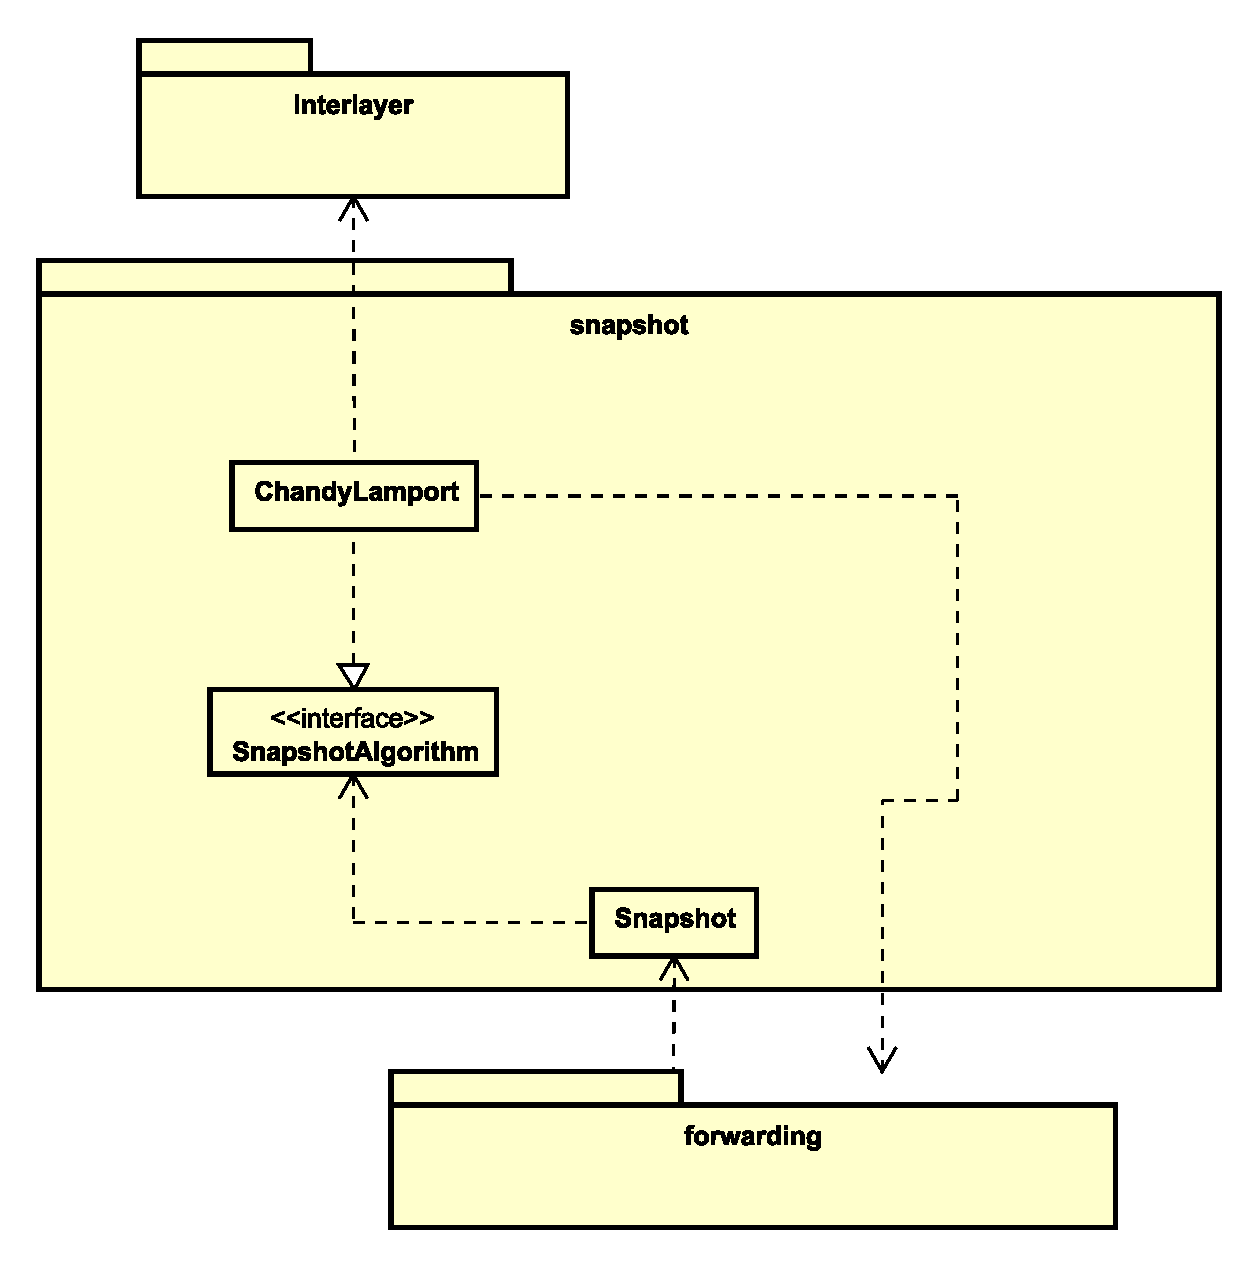
\includegraphics[width=\columnwidth]{images/solution/mw/snapshot.eps}
  \caption{Middleware's Snapshot service}
  \label{fig:mw-snapshot}
\end{figure}

% TODO: All class diagrams have to be added
\subsubsubsection{snapshot.Snapshot}
% TODO: Class diagram
\FloatBarrier
\begin{itemize}
  \item \textbf{Description} \\
    This module is the Fa\c cade of the Snapshot service. It is responsible
    to boot neatly and supervise all processes in Snapshot. Also, it has to
    handle snapshot requests that come from other nodes of the system.
  \item \textbf{Attributes}
  \item \textbf{Operations}
  \begin{itemize}
    \item \texttt{+ start()} \\
    Starts the Snapshot service.
    \item \texttt{+ handleMessage(message: String)} \\
    % TODO: check this out: Message will really be a String?
    Handles a snapshot start/termination request that comes from other nodes
    or receives snapshot information from the application layer.
  \end{itemize}
\end{itemize}

\subsubsubsection{snapshot.SnapshotAlgorithm}
% TODO: Class diagram
\FloatBarrier
\begin{itemize}
  \item \textbf{Description} \\
    Interface for processes that implement a certain kind of snapshot.
  \item \textbf{Attributes}
  \item \textbf{Operations}
  \begin{itemize}
    \item \texttt{+ take()} \\
    Starts to take a snapshot.
    \item \texttt{+ submitLocalSnapshot()} \\
    Stores a local snapshot.
    \item \texttt{+ submitRemoteSnapshot()} \\
    Stores a remote snapshot.
  \end{itemize}
\end{itemize}

\subsubsubsection{snapshot.ChandyLamport}
% TODO: Class diagram
\FloatBarrier
\begin{itemize}
  \item \textbf{Description} \\
    Module that implements the \texttt{snapshot.SnapshotAlgorithm}
    interface to take snapshots with the algorithm by Chandy and Lamport.
  \item \textbf{Attributes}
  \item \textbf{Operations}
  \begin{itemize}
    \item \texttt{+ take()} \\
    Starts to take a snapshot: that implies Forwarding module to notify
    other nodes of that and to hold messages until the snapshot is over; also
    that implies Interlayer to issue a snapshot request to the application
    layer.
    \item \texttt{+ submitLocalSnapshot()} \\
    Stores the snapshot of the node where the process is executing.
    \item \texttt{+ submitRemoteSnapshot()} \\
    Stores the snapshot of a remote node.
  \end{itemize}
\end{itemize}
